\section{Introduction}
This chapter presents a search for exotic decays of the Higgs boson to a pair of new (pseudo)scalar
particles, $H\to aa$, with a mass in the range 20--60 \GeV{}, and where one of the $a$ bosons decays into a pair of photons and the other to a pair of gluons.
The results of this search are published in~\cite{ref:TODO}.
The search is performed in event samples enhanced in vector-boson fusion Higgs boson production
by requiring two jets with large invariant mass in addition to the Higgs boson candidate decay products.
The analysis is based on the full dataset of $pp$ collisions at $\sqrt{s}= 13$ \TeV{} recorded in 2015 and 2016 with the ATLAS detector at the CERN Large Hadron Collider,
corresponding to an integrated luminosity of 36.7 \ifb.
The data are in agreement with the Standard Model predictions and an upper limit at the 95\% confidence level is placed on the production cross section times the
branching ratio for the decay $H\to aa\to \gamma\gamma gg$.
This limit ranges from 3.1 pb to 9.0 pb depending on the mass of the $a$ boson.


\section{Motivation}

%The search for the Standard Model (SM) Higgs 
%boson has been one of the main goals of the Large Hadron Collider (LHC) physics programme.  
%A Higgs boson with mass  of 125~\GeV, and with  properties compatible with those expected for the SM Higgs boson ($H$), 
%was discovered by the ATLAS~\cite{HIGG-2012-27} and CMS~\cite{CMS-HIG-12-028} collaborations.
%Since its discovery, a comprehensive programme of measurements of the properties of this particle has been underway.
%These measurements could uncover deviations from expected SM branching ratios or 
%set a limit on the possible branching ratio for decays into new particles beyond the SM (BSM).
%Existing measurements constrain the branching ratio for such decays ($B_\text{BSM}$) 
%to less than 34\% at 95\% confidence level (CL)~\cite{HIGG-2015-07}, 
%assuming that the absolute couplings to vector bosons are smaller than or equal to the SM ones.
%
%Many BSM models predict exotic decays of the Higgs boson~\cite{Curtin:2013fra}.
%One possibility is that the Higgs boson decays into a pair of 
%new (pseudo)scalar particles, $a$, which in turn decay to a pair of SM particles.
%Several searches have been performed for $H\to a a$ in various final 
%states~\cite{Abazov:2009yi,CMS-HIG-13-010,CMS-HIG-16-015,EXOT-2013-15,HIGG-2014-02}.
%
%The results presented in this chapter cover the unexplored $\gamma\gamma{jj}$ final state in searches for
%$H\to a a$, where one of the $a$ bosons decays into a pair of photons and the other decays into a pair of gluons.
%This final state becomes relevant in models where the fermionic decays are suppressed
%and the $a$ boson decays only into photons or gluons~\cite{Curtin:2013fra,hep-ph/0703247}.
%The ATLAS Run 1 search for $H\to aa \to \gamma\gamma\gamma\gamma$~\cite{EXOT-2013-24} set
%a 95\% CL limit $\sigma_H\times B(H\to aa\to \gamma\gamma\gamma\gamma)<10^{-3}~\sigma_\text{SM}$
%for $10<m_a<62~\GeV{}$, where $\sigma_\text{SM}$ is the production cross-section for the SM Higgs boson.
%There is currently no direct limit set on $B(H\to aa\to \gamma\gamma gg)$;
%however, in combination with $B_\text{BSM}<34\%$,
%the $H\to aa \to \gamma\gamma\gamma\gamma$ result sets an indirect limit on $B(H\to aa\to \gamma\gamma gg)$ to less than $\sim4\%$.
%Assuming the same ratio of photon and gluon couplings to the $a$ boson as to the SM Higgs boson,
%the $H\to \gamma\gamma\gamma\gamma$ decay occurs very rarely relative to the $H\to \gamma\gamma gg$ decay 
%(a typical value for the ratio $B(H\to \gamma\gamma\gamma\gamma)/B(H\to \gamma\gamma gg)$ is $3.8\times10^{-3}$~\cite{hep-ph/0703247})
%making $H\to \gamma\gamma jj$ an excellent unexplored final state for probing these fermion-suppressed coupling models.
%The branching ratio for $a\to \gamma\gamma$ can be enhanced in some scenarios.
%The two searches are therefore complementary,
%where the $H\to \gamma\gamma jj$ final state is more sensitive to photon couplings
%with the new physics sector similar to the photon coupling to the SM Higgs boson,
%while the $H\to \gamma\gamma\gamma\gamma$ final state is more sensitive to scenarios with enhanced photon couplings.
%
%Reference~\cite{hep-ph/0703247} shows that the search for $H \to \gamma\gamma gg$, 
%where the Higgs boson is produced in association with a vector boson which decays leptonically, 
%would require approximately $300~\ifb$ of LHC data in order to be sensitive to branching ratios less than 4\%. 
%The gluon--gluon fusion (ggF) production has a larger cross-section, 
%but is overwhelmed by the $\gamma\gamma$+multi-jet background.
%The strategy described in this chapter consists in selecting events where vector-boson fusion (VBF) is the dominant Higgs boson production mode.
%Even though the production rate is lower than that for the ggF mode, 
%the characteristic topology of the jets produced in association with the Higgs boson enables 
%more effective suppression of the background.

%%%%%%%%%%%

The search for the Standard Model (SM) Higgs 
boson~\cite{Englert:1964et,Higgs:1964pj,Higgs:1964ia,Guralnik:1964eu}  
has been one of the main goals of the LHC physics program.  
A new particle with mass  of 125 GeV, and with  properties compatible with those expected for the SM Higgs boson, 
has been discovered by the ATLAS~\cite{HIGG-2012-27} and CMS~\cite{CMS-HIG-12-028} collaborations.
Since its discovery, a comprehensive program of measurements of the properties of this particle has been underway.
These measurements could uncover deviations from expected SM branching ratios or 
allow for the possibility of decays into new particles. 
Existing measurements constrain the branching ratio for such decays ($\text{B}_\text{exotic}$) 
to less than 34\% at 95\% confidence level~\cite{Khachatryan:2016vau}.
Exotic decays are predicted by many theories of physics beyond the SM~\cite{Curtin:2013fra},
including those with an extended Higgs sector 
such as the Next-to-Minimal Supersymmetric Standard Model 
~\cite{Dobrescu:2000yn,Ellwanger:2003jt,Dermisek:2005ar,Chang:2008cw,Morrissey:2008gm},
several models of dark matter~\cite{SILVEIRA1985136,Pospelov:2007mp,Draper:2010ew,Ipek:2014gua,Martin:2014sxa},
models with a first order electroweak phase transition~\cite{Profumo:2007wc,Blinov:2015sna},
and theories with neutral naturalness~\cite{Burdman:2006tz,Craig:2015pha,Curtin:2015fna}.
These theories are motivated by some of the most outstanding unanswered questions in physics, such as the gauge hierarchy problem~\cite{Nilles:1982dy}, the nature of dark matter~\cite{Trimble:1987ee}, and the strong CP problem~\cite{Peccei:1977hh}.

One of the simplest possibilities is that the Higgs boson decays to a pair of 
new scalars or pseudoscalars, $a$, which in turn decay to a pair of SM particles.
Several searches have been performed for $H\rightarrow a a$ in various final states~\cite{Khachatryan:2017mnf,Aad:2015sva,Aad:2015oqa}.

The work presented here explores in particular the search for $H\rightarrow a a$, where the final state contains two photons ($\gamma$) and two gluons ($g$) ($H\rightarrow aa \rightarrow \gamma\gamma gg$).
This decay mode becomes relevant in models where the $a\rightarrow$ fermion decays are suppressed 
and the $a$ decays only to photons and gluons
~\cite{Curtin:2013fra,hep-ph/0703247}.
The ATLAS Run 1 search for $H\rightarrow aa \to 4\gamma$~\cite{Aad:2015bua} sets 
a limit $\sigma\times \text{B}(H\to aa\rightarrow 4\gamma)<10^{-3}\sigma_\text{SM}$ 
for $10~\GeV<m_a<62~\GeV$.
Before this work, there was no direct limit set on $\text{B}(H\rightarrow aa\rightarrow \gamma\gamma gg)$;
however, in combination with $\text{B}_\text{exotic}<34\%$, 
the $H\rightarrow 2a \to 4\gamma$ result sets indirect limits on $\text{B}(H\rightarrow aa\rightarrow \gamma\gamma gg)$ to less than $\sim4\%$ (Appendix~\ref{sec:HBSM_app:existinglimits}).
Assuming a SM-like ratio of photon and gluon couplings, 
the $H\rightarrow 4\gamma$ decay occurs very rarely relative to the $H\rightarrow \gamma\gamma gg$ decay (a typical value of the relative ratio of branching ratios is $3.8\times10^{-3}$~\cite{hep-ph/0703247})
\footnote{The $H\rightarrow 4g$ final state is the most common, but is unfortunately swamped by background.},
making the $H\rightarrow \gamma\gamma gg$ an excellent unexplored final state for probing these fermion-suppressed models.
The branching ratio for $a\rightarrow \gamma\gamma$ can be enhanced in some scenarios;
the two searches are therefore complementary, 
where the $H\rightarrow \gamma\gamma gg$ final state is more sensitive to SM-like photon couplings 
with the new physics sector, 
while the $H\rightarrow 4\gamma$ final state is more sensitive to the enhanced photon scenarios. 

The most common Higgs production modes at the LHC are through gluon fusion, vector boson fusion (VBF), or associated production with an additional vector boson (VH)~\cite{Dittmaier:2011ti}.
Ref.~\cite{hep-ph/0703247} shows that the search for $H \to \gamma\gamma gg$ in the VH mode, 
where the additional vector boson
decays leptonically, would require approximately $300~\ifb$ of LHC data in order to be sensitive to branching ratios less than 4\%. 
The gluon fusion production has a larger cross section, 
but is overwhelmed by background.
We have found (Fig.~\ref{fig:HBSM_prodmodes}) that the search in the VBF production 
mode can achieve sensitivity competitive with or better than the above two production modes in the range $20$ to $300~\ifb$ of LHC integrated luminosity data,
and in particular with the approximately $150~\ifb$ of data at the end of LHC Run 2~\cite{lhc-commissioning}.

In the VBF production mode, two extra quarks are produced along with the Higgs in the hard scatter interaction.
The gluons from the Higgs decay and the quarks from the VBF production are reconstructed as jets ($j$) in the ATLAS detector;
therefore, this search is focused on the $H\to2\gamma2j$ final state with two additional jets from the VBF production.
Fig.~\ref{fig:VBFH_feynman} shows a tree-level Feynman diagram of the VBF production and $\gamma\gamma gg$ decay of the Higgs boson, including the $aa$ intermediate state.

\begin{figure}[t]
  \centering 
  \subfloat[]{\includegraphics[width=0.45\textwidth]{figures/{HBSM_prodmodes}.pdf}\label{fig:HBSM_prodmodes}}
  \subfloat[]{
    \begin{tikzpicture}
      \begin{feynman}
        \vertex (q1init) {\(q\)};
        \vertex [below =4. of q1init] (q2init) {\(q\)};
        \vertex [below right=1. and 2. of q1init] (qqV);
        \vertex [above right=1. and 2. of q2init] (qqV2);
        \vertex [above right=1. and 4. of  qqV] (q1final) {\(q\)};
        \vertex [below right=1. and 4. of qqV2] (q2final) {\(q\)};
        \vertex [below right=1. and 1. of qqV] (VVH);
        \vertex [right=1. of VVH] (H);
        \vertex [above right=1. and 1. of H] (ayy);
        \vertex [below right=1. and 1. of H] (agg);
        \vertex [above right=0.5 and 1. of ayy] (y1) {\(\gamma\)};
        \vertex [below right=0.5 and 1. of ayy] (y2) {\(\gamma\)};
        \vertex [above right=0.5 and 1. of agg] (g1) {\(g\)};
        \vertex [below right=0.5 and 1. of agg] (g2) {\(g\)};
        \diagram* {
          (q1init) -- [fermion] (qqV) -- [fermion] (q1final),
          (q2init) -- [fermion] (qqV2) -- [fermion] (q2final),
          (qqV) -- [boson, edge label'=\(V\)] (VVH),
          (qqV2) -- [boson, edge label'=\(V\)] (VVH),
          (VVH) -- [scalar, edge label'=\(H\)] (H),
          (H) -- [scalar, edge label'=\(a\)] (ayy),
          (H) -- [scalar, edge label'=\(a\)] (agg),
          (ayy) -- [photon] (y1),
          (ayy) -- [photon] (y2),
          (agg) -- [gluon] (g1),
          (agg) -- [gluon] (g2),
        };
      \end{feynman}
    \end{tikzpicture}
    \label{fig:VBFH_feynman}
  }
  \caption{
    (a) Projected branching ratio for $H\rightarrow \gamma\gamma gg$ in order to make a discovery of new physics at a significance level of $5\sigma$, as a function of integrated luminosity, when searching in the gluon fusion (GGH), vector boson fusion (VBF), and associated production (VH) production modes.
    The projection for GGH and VBF assumes a $20\%$ systematic uncertainty due to jet reconstruction effects, while the projection for VH uses the estimation from Ref.~\cite{hep-ph/0703247}, assuming the significance is statistics-dominated.
    With less than $\sim 20 \ifb$, the gluon fusion mode is most sensitive, but with more statistics this production mode quickly becomes dominated by systematic uncertainties and is unable to provide better limits.
    Up to $\sim 300 \ifb$, the VBF mode is most sensitive; in Run 2 the LHC has gathered 140$\ifb$.
    With more than $\sim 300 \ifb$, the VH mode likely provides the best sensitivity.
    (b) Tree-level diagram of production and decay of Higgs boson being searched for in this analysis.
    }
\end{figure}

This search presents many interesting areas of original research in order to improve the sensitivity of the analysis.
The fully reconstructed final state contains four jets;
the main challenges present in this analysis involve reconstructing and identifying these jets.

When reconstructing the energy of the originating parton of a jet, both the effects of the energy response of the calorimeter and the effect of other proton-proton interactions in the event (pile-up) must be taken into account.
Chapter~\ref{ch:NI} presents work on studying in a rigorous framework the mathematical process of reversing the effects of the calorimeter response in order to access the originating parton energy (\cite{Cukierman:2016dkb});
and Chapter~\ref{ch:Calib} presents work on using machine learning to further improve this process.
Appendix~\ref{ch:Voronoi} presents work on novel jet reconstruction algorithms which aim to reduce the effect of pileup on the jet reconstructed energy~\cite{ATLAS-CONF-2017-065}.
These efforts serve to develop new techniques for reconstructing the energies of the jets that appear in the final state of this analysis, and therefore improve the ultimate sensitivity of this search.
These techniques can also be effective in the higher pileup conditions expected at the LHC in Run 3 and beyond, and are intended to be broadly applicable to other analyses than the one being studied here. 

\section{Data and simulation}

The search presented in this chapter is based on the 36.7~\ifb{} dataset of proton--proton collisions
recorded by the ATLAS experiment at the LHC at $\sqrt{s}=13$ \TeV{} during 2015 and 2016.
As discussed in Chapter~\ref{ch:ATLAS}, the ATLAS detector~\cite{PERF-2007-01} comprises an inner detector in a 2 T axial magnetic field, 
for tracking charged particles and a precise localisation of the interaction vertex, 
a finely segmented calorimeter, a muon spectrometer and a two-level trigger~\cite{TRIG-2016-01} that
accepts about 1 kHz rate for data storage.

Monte Carlo (MC) event generators were used to simulate the $H\to aa \to \gamma\gamma gg$ signal.
Signal samples for the ggF and VBF processes were generated at next-to-leading order using 
\POWHEGBOX{}~\cite{Nason:2004rx,Frixione:2007vw,Alioli:2010xd} interfaced with \PYTHIA{}~\cite{Sjostrand:2014zea} for parton showering and hadronisation using the AZNLO set of tuned parameters set~\cite{STDM-2012-23} and the CT10 parton distribution function (PDF) set~\cite{Lai:2010vv}.
Samples were generated in the $m_a$ range\footnote{The diphoton triggers considered for this
search do not have acceptance for the lower mass range ($m_a<20~\GeV{}$), where the two photons are collimated.} 
$20~\GeV{} < m_a < 60~\GeV{}$, assuming the $a$ boson to be a (pseudo)scalar.
All MC event samples were processed through a detailed simulation~\cite{SOFT-2010-01} of the ATLAS detector
based on \geantFour{}~\cite{Agostinelli:2002hh}, and contributions from additional $pp$ interactions (pile-up), simulated using
\PYTHIA{} and the MSTW2008LO PDF set~\cite{Martin:2009iq}, were overlaid onto the hard-scatter events.

\section{Event Selection}
\subsection{Trigger}
Events are selected by two diphoton triggers.
One trigger path requires the presence in the electromagnetic (EM) calorimeter of two clusters of energy
deposits with transverse energy
%\footnote{ATLAS uses a right-handed coordinate system with its origin at the nominal interaction point (IP) in the centre of the detector and the $z$-axis along the beam pipe. The $x$-axis points from the IP to the centre of the LHC ring, and the $y$-axis points upward. Cylindrical coordinates $(r,\phi)$ are used in the transverse plane, $\phi$ being the azimuthal angle around the $z$-axis. The pseudorapidity is defined in terms of the polar angle $\theta$ as $\eta=-\ln\tan(\theta/2)$.}
above 35 \GeV{} and 25 \GeV{} for the leading (highest transverse energy) and sub-leading
(second-highest transverse energy) clusters, respectively. In the high-level trigger the shape of the energy
deposit in both clusters is required to be loosely consistent with that expected from an EM shower initiated by a photon.
The other trigger path requires the presence of two clusters with transverse energy above 22 \GeV{}.
In order to suppress the additional rate due to the lower transverse energy threshold, the shape requirements for the energy deposits are
more stringent.

\subsection{Photons}
The photon candidates are reconstructed from the clusters of energy deposits in the EM calorimeter within the range $|\eta|<2.37$.
The energies of the clusters are calibrated to account for energy losses upstream of the calorimeter 
and for energy leakage outside the cluster, as well as other effects due to the detector geometry and response.
The calibration is refined by applying $\eta$-dependent correction factors of the order of $\pm1$\%, derived from $Z\to ee$ events~\cite{PERF-2013-05}.
As in the trigger selection, photon candidates are required to satisfy a set of identification criteria based on the shape of the EM cluster~\cite{PERF-2013-04}.
Two working points are defined: a \textit{Loose} working point, used for the preselection and the data-driven background estimation, and a 
\textit{Tight} working point, with requirements that further reduce the misidentification of neutral hadrons decaying to two photons.
In order to reject the hadronic jet background, photon candidates are required to be isolated from any other activity in the calorimeter.
The calorimeter isolation is defined as the sum of the transverse energy in the
calorimeter within a cone of \mbox{$\Delta R = \sqrt{(\Delta\eta)^2+(\Delta\phi)^2}=0.4$} centred around the photon candidate,
The transverse energy of the photon candidate is subtracted from the calorimeter isolation.
Contributions to the calorimeter isolation from the underlying event and pile-up are subtracted using the method proposed in Ref.~\cite{jetareas}.
Candidates with a calorimeter isolation larger than 2.2\% of the photon's transverse energy are rejected.

Events are required to have at least two photon candidates. 
The transverse energy requirements depend on the trigger path through which the event was recorded.
For events passing the trigger with higher transverse energy thresholds, the leading photon is required to have $E_\text{T}>40$ \GeV{}, 
and the sub-leading photon is required to have $E_\text{T}>30$ \GeV{}. For events passing the trigger with lower thresholds, 
both the leading and sub-leading photons are required to have $E_\text{T}>27$ \GeV{}. 
For events passing both triggers, the latter selection is applied.
The invariant mass of the two leading photon candidates is denoted by $m_{\gamma\gamma}$.
The $m_{\gamma\gamma}$ resolution is excellent at less than $2$ \GeV{}, as can be seen in Fig.~\ref{fig:HBSM:photon_kinematics}.

\begin{figure}[htbp]
  \centering 
  \subfloat[]{\includegraphics[width=0.45\textwidth]{figures/{myy_unscaled_combine_ma_VBF8_8.7.17}.pdf}\label{fig:myy_unscaled}}
  \subfloat[]{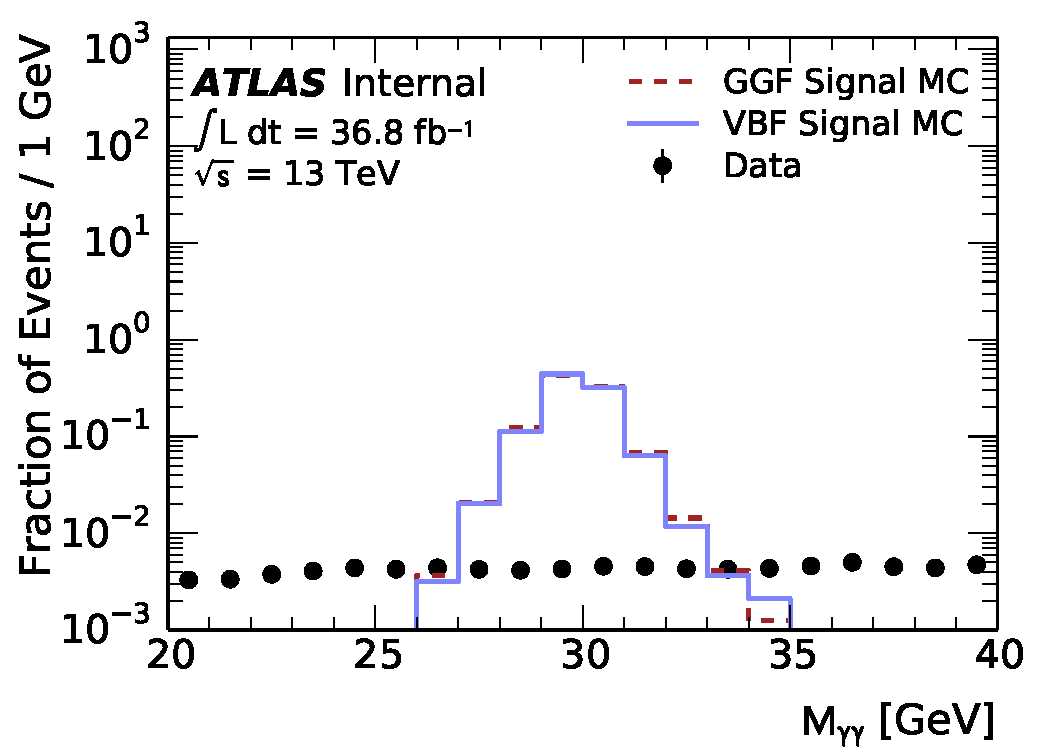
\includegraphics[width=0.45\textwidth]{figures/myy_shape_log.pdf}}\\
  \caption{Distribution of $m_{\gamma\gamma}$. The quantities are plotted separately for signal MC produced in the VBF and GGF modes. (a) The distribution for all the signal samples used in this analysis (each signal normalized to a branching ratio BR($H\rightarrow aa \rightarrow \gamma\gamma jj)=0.03$). (b) Zoomed in distribution, for a signal with $m_a=30$ GeV.}
  \label{fig:HBSM:photon_kinematics}
\end{figure}

\subsection{Jets}
Jets are reconstructed from topological clusters~\cite{PERF-2014-07} using the anti-$k_t$
algorithm~\cite{Cacciari:2008gp} implemented in the FastJet package~\cite{Cacciari:2011ma} with a radius parameter of $R=0.4$. 
Jets are calibrated using an energy- and $\eta$-dependent
calibration scheme, and are required to have a transverse momentum (\pt{}) greater than $20~\GeV{}$ and $|\eta|<2.5$ or $\pt>30~\GeV{}$ and $|\eta|<4.4$.
A track- and topology-based veto~\cite{PERF-2014-03,PERF-2016-06} is used to suppress jets originating from pile-up interactions.
Jets must have an angular separation of $\Delta R>0.4$ from any \textit{Loose} photon candidate in the event.

\subsection{VBF Selection}
\label{sec:HBSM:VBF_sel}
In the VBF production mode, the Higgs boson is produced in association with two additional light-quark jets
with a large opening angle and a large invariant mass.
Selected events are therefore required to have at least four jets and 
the pair of jets with the highest invariant mass ($m_{jj}^\text{VBF}$, or \textit{VBF $m_{jj}$}) are referred to as \textit{VBF jets}.
The two remaining highest-\pt{} jets are referred to as \textit{signal jets}, with invariant mass $m_{jj}$.
The jet assignment is designed to choose the correct VBF and signal jets for VBF signal events. The truth parton label (the truth ID of the highest $p_T$ parton in the jet) is used to study the accuracy of this jet assignment in MC.

As seen in Fig.~\ref{fig:numIDjets}, after the 4 jet preselection requirement, about 70\% of VBF signal events contain at least 2 gluon jets; also, about 70\% of VBF signal events contain at least 2 quark jets. This limits the possible accuracy of the jet assignment.

\begin{figure}[htbp]
  \centering 
  \subfloat[]{\includegraphics[width=0.45\textwidth]{figures/{VBF7_numgluonjets_4j_VBF_a30_ggyy_6.21.17_Nominal}.pdf}}
  \subfloat[]{\includegraphics[width=0.45\textwidth]{figures/{VBF7_numquarkjets_4j_VBF_a30_ggyy_6.21.17_Nominal}.pdf}}
  \caption{Jet multiplicity of (a) gluon and (b) quark jets in a VBF signal sample with $m_a=30$ GeV.}
  \label{fig:numIDjets}
\end{figure}

The best possible jet assignment would choose the two gluon jets with mass closest to $m_a$ as the signal jets and two quark jets as the VBF jets, if such an assignment is possible.
Fig.~\ref{fig:truegluon} shows the results of this assignment (which can only be done at truth level) for a VBF signal sample with $m_a=30$ GeV.

In the $m_{jj}$ distribution there is a peak about $m_a$ with width about $0.4m_a = 12$ GeV.
Only about 35\% of the events have two gluons with an invariant mass within this peak; this indicates that most of the time the two true signal gluons are either not reconstructed or below the jet $p_T$ cut.
This 12 GeV width also informs the choice of a $0.4m_a$ cut on $|m_{jj}-m_{\gamma\gamma}|$ in the ABCD regions definition (\ref{sec:HBSM:signal_selection}).

\begin{figure}[htbp]
  \centering 
  \subfloat[]{\includegraphics[width=0.45\textwidth]{figures/{VBF7_count_ids_bar_true_gluon_signal_VBF_a30_ggyy_6.21.17_Nominal}.pdf}}
  \subfloat[]{\includegraphics[width=0.45\textwidth]{figures/{VBF7_mjj_true_gluon_signal_VBF_a30_ggyy_6.21.17_Nominal}.pdf}}
  \caption{(a) Truth parton label of jets chosen as signal jets in a VBF signal sample with $m_a=30$ GeV; the jet assignment is to choose the two truth gluons with mass closest to $m_a$ as the signal jets and the two highest $p_T$ truth quark jets as the VBF jets, if such an assignment is possible (i.e., this assignment can only be done at truth level). (b) The distribution of $m_{jj}$ for the signal jets.}
  \label{fig:truegluon}
\end{figure}

Fig.~\ref{fig:remove} shows the results of the jet assignment used in this analysis for a VBF signal sample with $m_a=30$ GeV.
About 20\% of the events choose two gluons with an invariant mass within 12 GeV of $m_a$ as the signal jets.
About 55\% of the events choose two quarks correctly as the VBF jets.

Fig.~\ref{fig:VBFmjj_quarkquark} examines the distribution of VBF $m_{jj}$ with the jet assignment used in this analysis in a VBF signal sample with $m_a=30$ GeV using truth information.
The distributions are compared among all events, events where both VBF jets are truth identified as quarks, and events where at least one VBF jet is not truth identified as a quark.
It can be seen that the VBF $m_{jj}$ distribution is shifted upwards relative to the case where the truth quarks are not correctly selected, but the case where the truth quarks are always correctly selected is shifted to even higher values.

Fig.~\ref{fig:remove} also shows the results of the jet assignment used in this analysis for a gluon fusion signal sample with $m_a=30$ GeV and for a photons + jets background MC sample.
In the gluon fusion signal sample, about 20\% of the events choose two gluons with an invariant mass within 12 GeV of $m_a$ as the signal jets.
In these events the jets labeled the ``VBF jets" in fact come from pileup, underlying event, or initial or final state radiation. 

\begin{figure}[htbp]
  \centering 
  \subfloat[]{\includegraphics[width=0.45\textwidth]{figures/{VBF7_count_ids_bar_remove_VBF_a30_ggyy_6.21.17_Nominal}.pdf}}
  \subfloat[]{\includegraphics[width=0.45\textwidth]{figures/{VBF7_count_ids_bar_remove_VBFID_VBF_a30_ggyy_6.21.17_Nominal}.pdf}}\\
  \subfloat[]{\includegraphics[width=0.45\textwidth]{figures/{VBF7_count_ids_bar_remove_ggH_a30_ggyy_6.21.17_Nominal}.pdf}}
  \subfloat[]{\includegraphics[width=0.45\textwidth]{figures/{VBF7_count_ids_bar_remove_VBFID_ggH_a30_ggyy_6.21.17_Nominal}.pdf}}\\
  \subfloat[]{\includegraphics[width=0.45\textwidth]{figures/{VBF7_count_ids_bar_remove_myy_0_55_7.6.17_Nominal}.pdf}}
  \subfloat[]{\includegraphics[width=0.45\textwidth]{figures/{VBF7_count_ids_bar_remove_VBFID_myy_0_55_7.6.17_Nominal}.pdf}}\\
  \caption{Truth parton label of jets chosen as (a) signal jets and (b) VBF jets in a VBF signal sample with $m_a=30$ GeV; (c) signal jets and (d) VBF jets in a gluon fusion signal sample with $m_a=30$ GeV; and (e) signal jets and (f) VBF jets in a photons + jets background sample.}
  \label{fig:remove}
\end{figure}

\begin{figure}[htbp]
  \centering 
  \subfloat[]{\includegraphics[width=0.45\textwidth]{figures/{vbf_mjj_truthid_shape}.pdf}}
  \caption{Comparison of distribution of VBF $m_{jj}$ with the jet assignment used in this analysis in a VBF signal sample with $m_a=30$ GeV. The comparison is between the distribution for all events; the distribution for events where both jets identified as VBF jets are truth labeled as quark jets; and the distribution for events where at least one jet identified as as a VBF jet is not truth labeled as a quark jet.}
  \label{fig:VBFmjj_quarkquark}
\end{figure}

The VBF Higgs boson signal is further enhanced,
relative to the dominant $\gamma\gamma$+multi-jet background,
by requiring $m_{jj}^\text{VBF}$ to be greater than 500 \GeV{} and 
the \pt{} of the leading VBF jet to be greater than 60 \GeV{}.
The discrimination power of these observables can be seen in the difference in shape between the VBF signal and the 
data, shown in Fig.~\ref{fig:HBSM:VBF_jet_kinematics}.

\begin{figure}[t]
  \centering 
  \subfloat[]{\includegraphics[width=0.45\textwidth]{figures/{vbf_mjj_shape_log_VBF8_combined_8.7.17}.pdf}}
  \subfloat[]{\includegraphics[width=0.45\textwidth]{figures/{vbf_jet1pt_postselection_shape_log_VBF8_combined_8.7.17}.pdf}}\\
  \caption{
    Distributions of kinematic observables before the requirements on \smash{$m_{jj}^\text{VBF}$}, leading VBF jet \pt{}, \smash{$m_{\gamma\gamma jj}$}
    and $|m_{jj}-m_{\gamma\gamma}|$ for:
    (a) $m_{jj}^\text{VBF}$; and (b) leading VBF jet \pt{}.
    The quantities are shown separately for simulated signal events (with $m_a=30$ \GeV{}) produced in the VBF mode 
    and compared with those produced in the ggF mode and the observed data.
    }
  \label{fig:HBSM:VBF_jet_kinematics}
\end{figure}

\subsection{Signal Selection}
\label{sec:HBSM:signal_selection}
As mentioned in~\ref{sec:HBSM:VBF_sel}, the two remaining highest-\pt{} jets after the VBF jet assignment are referred to as \textit{signal jets}, with invariant mass $m_{jj}$.
The distribution of $m_{jj}$ is shown in Fig.~\ref{fig:HBSM:signal_kinematics}; the resolution is quite broad, on the order of 30\% of the central value.
The tail of the $m_{jj}$ distribution comes from misidentifying the signal jets.
The distribution of $|m_{jj}-m_{\gamma\gamma}|$ is also shown in Fig.~\ref{fig:HBSM:signal_kinematics}; 
for $H\to aa \to \gamma\gamma gg$ signal events, where the $a$ boson candidates have similar masses, the difference $|m_{jj}-m_{\gamma\gamma}|$ tends to be smaller.
This quantity is therefore used to define a signal-enhanced region for the data-driven background estimation (Section~\ref{sec:HBSM:background_est}).

The two photon candidates and the two signal jets form the Higgs boson candidate with invariant mass $m_{\gamma\gamma jj}$, 
which is required to be in the range $100 < m_{\gamma\gamma jj} < 150~\GeV{}$. 
Figure~\ref{fig:HBSM:signal_kinematics} shows that most of the selected signal events lie within this range, especially after the requirement of $|m_{jj}-m_{\gamma\gamma}|$ used to define the signal-enhanced region,
while the data have a broad distribution extending to higher values.

\begin{figure}[t]
  \centering 
  \subfloat[]{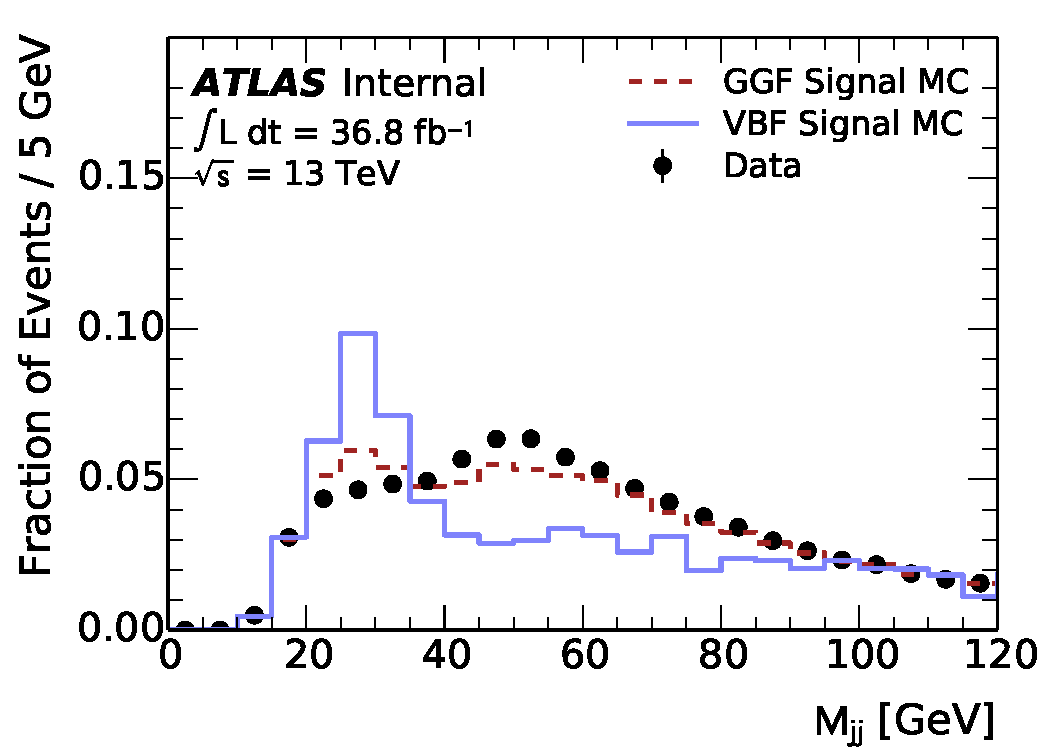
\includegraphics[width=0.45\textwidth]{figures/mjj_shape.pdf}}
  \subfloat[]{\includegraphics[width=0.45\textwidth]{figures/{amassdiff_shape_VBF8_combined_8.7.17}.pdf}}\\
  \subfloat[]{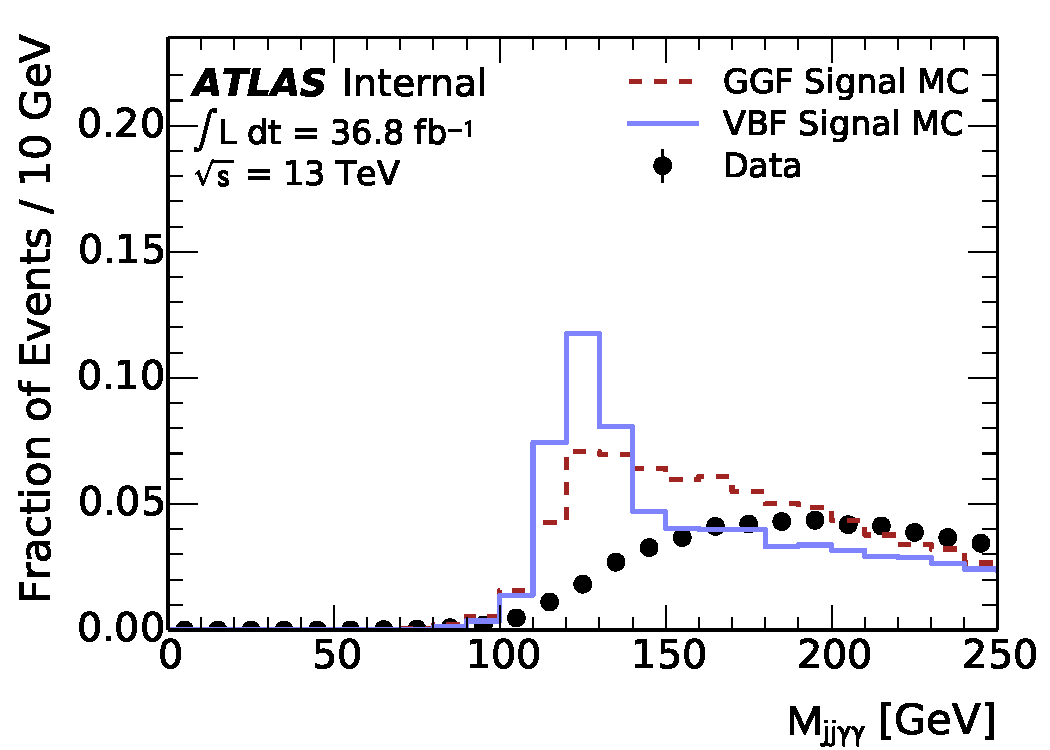
\includegraphics[width=0.45\textwidth]{figures/hmasses_shape.pdf}}
  \subfloat[]{\includegraphics[width=0.45\textwidth]{figures/{hmass_amassdiff_shape_VBF8_combined_8.7.17}.pdf}}\\
  \caption{
    Distributions of kinematic observables before the requirements on \smash{$m_{jj}^\text{VBF}$}, leading VBF jet \pt{}, \smash{$m_{\gamma\gamma jj}$}
    and $|m_{jj}-m_{\gamma\gamma}|$ for:
    (a) $m_{jj}$;
    (b) $|m_{jj}-m_{\gamma\gamma}|$;
    (c) $m_{\gamma\gamma jj}$;
    and (d) $m_{\gamma\gamma jj}$ (with the additional requirement $|m_{jj}-m_{\gamma\gamma}|< 12~\GeV{}$ that defines the signal-enriched region).
    The quantities are shown separately for simulated signal events (with $m_a=30$ \GeV{}) produced in the VBF mode 
    and compared with those produced in the ggF mode and the observed data.
    }
  \label{fig:HBSM:signal_kinematics}
\end{figure}

In order to take advantage of the very good $m_{\gamma\gamma}$ resolution to suppress the background with $m_{\gamma\gamma}$ far from the
range of interest, five overlapping $m_{\gamma\gamma}$ regimes are defined as summarised in Table~\ref{tab:amassdiffcut}.
The boundaries of the $m_{\gamma\gamma}$ regimes are chosen so that for any value of $m_a$ 
considered in the scope of this search there is at least one regime where there is no significant signal acceptance loss
due to the $m_{\gamma\gamma}$ requirement.
For each $m_{\gamma\gamma}$ regime, the set of $m_a$ values for which this requirement causes no significant signal acceptance loss is also indicated.

\section{Background estimation}
\label{sec:HBSM:background_est}
The $\gamma\gamma$+multi-jet background consists of multi-jet events with two reconstructed photon candidates, 
originating from isolated EM radiation or from jets.
A data-driven estimation based on two-dimensional sidebands is used to predict the background yields.
The method consists of using two uncorrelated observables
to define four regions labelled A, B, C and D.

The first axis of the A/B/C/D plane separates events in regions C and D with both photons passing the \textit{Tight} requirement 
from events in regions A and B with at most one photon 
passing the \textit{Tight} requirement and at least one passing the \textit{Loose} but not the \textit{Tight} requirement. 
These regions are referred to respectively as \textit{Tight--Tight} (C and D) and \textit{Tight--Loose} (A and B). 

The second axis separates events in regions B and D, satisfying $|m_{jj}-m_{\gamma\gamma}|< x_\text{R}$, 
from events in regions A and C, satisfying $|m_{jj}-m_{\gamma\gamma}|>x_\text{R}$. 
The value $x_\text{R}$ depends on the $m_{\gamma\gamma}$ regime R to account for the degradation in resolution at higher mass.
As mentioned in Section~\ref{sec:HBSM:signal_selection}, the difference $|m_{jj}-m_{\gamma\gamma}|$ tends to be smaller in the signal than in the background.
The signal events that lie outside of the range $|m_{jj}-m_{\gamma\gamma}|< x_\text{R}$ are due to poor $m_{jj}$ resolution or to incorrect assignment of the jets corresponding 
to the gluons originating from the $a$ boson decay.
Specific $x_\text{R}$ values are given in Table~\ref{tab:amassdiffcut}.
In each $m_{\gamma\gamma}$ regime, the boundary for $|m_{jj}-m_{\gamma\gamma}|$ is 0.4 times the central $m_{\gamma\gamma}$ value.
An exception is made for the lowest $m_{\gamma\gamma}$ regime, where $x_\text{R}$ is larger in order to increase the signal efficiency.

\begin{table}[t]
  \begin{center}
    \caption{
      Definition of each $m_{\gamma\gamma}$ regime, the range of $m_a$ values considered in the scope of this search with no significant signal loss acceptance due to the $m_{\gamma\gamma}$ requirement, and the corresponding boundary $x_\text{R}$ for $|m_{jj}-m_{\gamma\gamma}|$.  
    }
  \label{tab:amassdiffcut}
    {\footnotesize
  \begin{tabular}{ c c c c }
    \toprule
    $m_{\gamma\gamma}$ regime & Definition & Range of $m_a$ values & $x_\text{R}$ [\GeV{}] \\
    \midrule
    1 & $17.5$ \GeV{} $< m_{\gamma\gamma}< 27.5$ \GeV{} & $20$ \GeV{} $\le m_a \le 25$ \GeV{} & 12 \\
      2 & $22.5$ \GeV{} $< m_{\gamma\gamma}< 37.5$ \GeV{} & $25$ \GeV{} $\le m_a \le 35$ \GeV{} & 12 \\
      3 & $32.5$ \GeV{} $< m_{\gamma\gamma}< 47.5$ \GeV{} & $35$ \GeV{} $\le m_a \le 45$ \GeV{} & 16 \\
      4 & $42.5$ \GeV{} $< m_{\gamma\gamma}< 57.5$ \GeV{} & $45$ \GeV{} $\le m_a \le 55$ \GeV{} & 20 \\
      5 & $52.5$ \GeV{} $< m_{\gamma\gamma}< 65.0$ \GeV{} & $55$ \GeV{} $\le m_a \le 60$ \GeV{} & 24 \\
    \bottomrule
  \end{tabular}
    }
  \end{center}
\end{table}

Region D is expected to contain the highest contribution of signal. 
In this region, 60\% of the signal events are produced in the VBF mode and the remaining 40\% in the ggF mode.
Assuming no correlation in the background events between the two observables used to define the A/B/C/D regions,
the number of background events in the signal region D ($N^\text{bkg}_\text{D}$) is related to the number
of background events in the control regions A, B and C, denoted by $N^\text{bkg}_\text{A}$, $N^\text{bkg}_\text{B}$
and $N^\text{bkg}_\text{C}$, respectively, by the formula
\begin{align}
N^\text{bkg}_\text{D} = \frac{N^\text{bkg}_\text{B}N^\text{bkg}_\text{C}}{N^\text{bkg}_\text{A}}.
\label{eqn:closure}
\end{align}
In the following, the difference between the prediction $N^\text{bkg}_\text{D}$ and the actual background yield in region D 
is referred to as \textit{non-closure}.
The non-closure results from residual correlations between the two observables used to define the A/B/C/D regions,
and the uncertainty accounting for this effect is referred to as \textit{closure uncertainty}.
In order to quantify the non-closure, the data-driven estimation as described above is performed 
with the exception that the requirement on $m_{\gamma\gamma jj}$ is inverted.
For each $m_{\gamma\gamma}$ regime,
the closure uncertainty is defined to be 
the central value of the non-closure if it is found to be significant ($>1\sigma$) in comparison with its statistical uncertainty; 
otherwise, the statistical uncertainty of its estimate is used.

\section{Results}

The efficiency of the event selection for the $pp\to H\to aa \to \gamma\gamma gg$ signal in each of the A/B/C/D regions is shown in Table~\ref{tab:ABCD},
assuming the SM cross-section and kinematics for the different production modes as described in Ref.~\cite{deFlorian:2016spz}.
The observed number of events in each of the A/B/C/D regions for each $m_{\gamma\gamma}$ regime is shown in Table~\ref{tab:ABCD_data}
along with the predicted background in the signal region D, taking into account the closure uncertainty. 
Due to the low event counts in each of the A/B/C/D regions,
the median expected background yield in region D estimated from pseudo-data experiments involving asymmetric Poisson uncertainties 
in the different regions slightly differs from the direct estimation from Eq.~(\ref{eqn:closure}).
No large excess is observed in region D when comparing the data yield to the background predicted from the A/B/C regions
assuming that the signal is absent in these regions.
However, given that a signal contamination is possible, a more refined procedure
taking into account signal contributions in all regions
is employed to set limits on the production rate of $H\to aa \to \gamma\gamma gg$.

\begin{table}[t]
  \begin{center}
    \caption{Efficiency of event selection on the $pp\to H\to aa \to \gamma\gamma gg$ signal, 
      assuming the SM Higgs boson production cross-section and kinematics,
      in each of the A/B/C/D regions, for different $m_a$ mass hypotheses.
      For each $m_a$ value, all $m_{\gamma\gamma}$ regimes in which there is no significant signal acceptance loss due to the $m_{\gamma\gamma}$ requirement are shown.
    }
    \label{tab:ABCD}
    \footnotesize
    \bgroup
    \def\arraystretch{1.5}
    \begin{tabular}{
        c
        c
        r@{}l
        r@{}l
        r@{}l
        r@{}l
      }
      \hline
      {$m_a$ [\GeV{}]} & {$m_{\gamma\gamma}$ regime} & \multicolumn{8}{c}{Efficiency $(\times 10^{-5})$}  \\
      & & \multicolumn{2}{c}{A} & \multicolumn{2}{c}{B} & \multicolumn{2}{c}{C} & \multicolumn{2}{c}{D}  \\
      \hline
      20 & 1 & 0.50&$^{+0.16}_{-0.14}$ & 1.2&$\pm0.4$ & 3.9&$\pm1.1$           & 6.2&$\pm1.8$           \\
      25 & 1 & 0.67&$^{+0.27}_{-0.33}$ & 2.6&$^{+0.5}_{-0.6}$ & 5.8&$\pm1.4$           & 15&$\pm4$           \\ 
      25 & 2 & 0.67&$^{+0.27}_{-0.33}$ & 2.6&$^{+0.5}_{-0.6}$ & 5.8&$\pm1.4$           & 15&$\pm4$           \\ 
      30 & 2 & 1.22&$\pm0.34$           & 3.3&$\pm0.9$          & 7.6&$^{+1.4}_{-1.6}$   & 25&$^{+5}_{-6}$   \\
      35 & 2 & 1.8&$\pm1.1$            & 2.7&$\pm1.2$           & 9.3&$\pm2.6$           & 27&$\pm6$           \\ 
      35 & 3 & 0.53&$^{+1.20}_{-0.24}$  & 4.1&$\pm1.2$           & 6.1&$^{+1.2}_{-1.6}$   & 31&$\pm7$           \\
      40 & 3 &  1.2&$\pm0.4$           & 3.3&$\pm1.0$           & 7.9&$^{+1.7}_{-2.4}$   & 26&$\pm6$           \\
      45 & 3 & 2.5&$\pm1.0$           & 4.1&$\pm1.3$           & 7.7&$^{+1.7}_{-2.0}$   & 19&$\pm5$           \\ 
      45 & 4 & 2.2&$\pm0.9$  & 4.4&$\pm1.4$           & 5.9&$^{+1.5}_{-2.2}$   & 22&$\pm5$           \\ 
      50 & 4 &  0.93&$\pm0.30$           & 4.4&$\pm1.2$           & 5.0&$^{+1.3}_{-1.0}$   & 24&$\pm5$   \\
      55 & 4 & 0.37&$\pm0.11$          & 3.3&$\pm0.9$          & 5.4&$^{+1.3}_{-1.4}$   & 21&$\pm5$           \\ 
      55 & 5 & 0.23&$\pm0.16$          & 3.6&$\pm1.0$          & 3.4&$\pm0.8$          & 24&$\pm6$           \\ 
      60 & 5 &  0.77&$^{+0.32}_{-0.30}$  & 3.9&$\pm1.0$           & 4.9&$\pm1.4$           & 23&$\pm6$           \\
      \hline
    \end{tabular}
    \egroup
  \end{center}
\end{table}

\begin{table}[t]
  \begin{center}
    \caption{Number of events observed in each of the A/B/C/D regions, 
      the relative size of the closure uncertainty considered for each $m_{\gamma\gamma}$ regime, 
      and the prediction for the number of background events in region D based on the control region yields.
      The median predicted background yield and its $\pm1\sigma$ uncertainty in region D is also shown.
      The uncertainties in the prediction account for both the Poisson fluctuations of the number of events in the control regions 
      and the closure uncertainty.
    }
    \label{tab:ABCD_data}
          {\footnotesize
            \bgroup
            \def\arraystretch{1.3}
	    \begin{tabular}{
                ccccccr@{}l
              }
	      \hline
              $m_{\gamma\gamma}$ regime &   A &   B &   C &   D  & Relative closure uncert. & \multicolumn{2}{c}{Predicted background yield}\\
	      \hline
              1 &  15 &   4 &  28 &   4 &  0.50 & \hspace{1.4cm}6&$^{+7}_{-4}$   \\
              2 &  22 &   6 &  34 &  15 &  0.32 & 8&$^{+7}_{-4}$   \\
              3 &  12 &  16 &  29 &  26 &  0.20 & 37&$^{+23}_{-14}$ \\
              4 &   8 &  12 &  19 &  38 &  0.21 & 27&$^{+22}_{-12}$ \\
              5 &   6 &  20 &  20 &  36 &  0.20 & 66&$^{+56}_{-28}$ \\
	      \hline
	    \end{tabular}
            \egroup
          }
  \end{center}
\end{table}

A likelihood function, describing both the expected background and signal, is fit to all four A/B/C/D regions simultaneously.
The free parameters of the likelihood are the numbers of signal and background events in region D, 
$\mu_\text{S}$ and $\mu_\text{bkg}$ respectively, the ratio of background events expected in region B to that in region D, $\tau_\text{B}$, 
and the analogous ratio for region C, $\tau_\text{C}$.
The assumption of no correlation in the total background, Eq.~(\ref{eqn:closure}), 
allows the background to be parameterised in terms of only three parameters.
The closure uncertainty, which accounts for the uncertainty due to assuming non-correlation, is included in the likelihood function by applying a Gaussian prior
to the expected number of background events in region A, $\tau_\text{B}\tau_\text{C}\mu_\text{bkg}$.
The Gaussian width is determined by the size of the closure uncertainty summarized in Table~\ref{tab:ABCD_data}.
The parameter $\mu_\text{S}$ can be expressed as the product of the total integrated luminosity, the signal cross-section 
$\sigma_H\times B(H\to aa\to \gamma\gamma gg)$, and the signal selection efficiency estimated in MC simulation
and quoted in Table~\ref{tab:ABCD}.
The signal contamination in the control regions A, B, and C is estimated from MC simulation 
and is varied coherently with $\mu_\text{S}$ in the likelihood fit.

The low number of observed events is the dominant source of uncertainty for this search.
The second largest uncertainty is due to the closure uncertainty, also statistical in nature.
Other sources of systematic uncertainty only affect the overall signal normalisation and the amount of signal contamination
in control regions A, B and C.
Dominant sources of experimental systematic uncertainty arise from the calibration and resolution of the energy of the 
jets~\cite{PERF-2016-04,PERF-2011-04}. 
Uncertainties associated with the photon energy calibration and resolution~\cite{PERF-2013-05}, as well as the photon identification and isolation
efficiencies~\cite{PERF-2013-04}, are found to be negligible. Uncertainties associated 
with the estimation of the integrated luminosity and the simulation of pile-up interactions (\textit{Lumi and Pile-up})
are found to be negligible. 
The systematic uncertainty associated with the modelling of the kinematics in signal 
events (\textit{Modelling}) is evaluated by varying the choice of scales used in the generator program and
assuming the SM Higgs boson production~\cite{Heinemeyer:2013tqa}.
It is found to be similar in size to the experimental systematic uncertainty.

Nuisance parameters corresponding to each source of uncertainty are included in the profile likelihood as Gaussian constraints.
Their effects on the estimated number of signal events $\mu_\text{S}$ are studied using Asimov~\cite{Cowan:2010js} pseudo-datasets generated
for an expected signal corresponding to the 95\% CL upper limit obtained in this search and using the values of the background 
parameters maximising the likelihood in a fit to data which assumes no signal.
Table~\ref{tab:systs} summarises the impact of each source of uncertainty varied by $\pm1\sigma$ on the maximum-likelihood estimate for $\mu_\text{S}$ in each 
of the $m_{\gamma\gamma}$ regimes for an illustrative $m_a$ hypothesis. The statistical uncertainty is the largest one for all regimes.
\begin{table}[t]
  \begin{center}
    \caption{
      Maximum fractional impact on the fitted $\mu_\text{S}$ from sources of systematic uncertainty estimated using Asimov datasets.
      The signal injected in the Asimov datasets corresponds to the observed upper limit quoted in Table~\ref{tab:limits}.
    }
    \label{tab:systs}
          {\footnotesize
	  \begin{tabular}{cccccc}
	  \hline
          &\multicolumn{5}{c}{$m_{\gamma\gamma}$ regime} \\
          Source of Uncert.   &    1  &   2  &   3  &   4  &   5  \\
            &   $m_a=20~\GeV{}$ &  $m_a=30~\GeV{}$ &  $m_a=40~\GeV{}$ &  $m_a=50~\GeV{}$ &  $m_a=60~\GeV{}$ \\
          \hline
	  Statistical          &     0.73 &     0.51 &     0.89 &     1.13 &     0.92 \\
	  Closure              &     0.44 &     0.27 &     0.39 &     0.64 &     0.89 \\
	  \hline
	  Modelling            &     0.35 &     0.34 &     0.46 &     0.42 &     0.65 \\
	  Jet                  &     0.58 &     0.38 &     0.25 &     0.90 &     0.71 \\
	  Photon               &     0.06 &     0.05 &     0.10 &     0.12 &     0.13 \\
	  Lumi and Pile-up     &     0.06 &     0.04 &     0.27 &     0.14 &     0.32 \\
	  \hline
	  \end{tabular}
          }
  \end{center}
\end{table}
The best-fit values of the parameters of the likelihood function are given in Table~\ref{tab:MLE}.
The probability that the data are compatible with the background-only hypothesis is computed for each $m_{\gamma\gamma}$ regime and no significant 
excess is observed. The smallest local $p$-value, obtained for the $m_{\gamma\gamma}$ regime 2 ($m_a\approx30~\GeV{}$), is of the order of 4\%.
\begin{table}[t]
  \begin{center}
    \caption{Maximum-likelihood fit values for each of the free parameters of the likelihood function 
      in each $m_{\gamma\gamma}$ regime for a relevant signal $m_a$ hypothesis.
      The estimated uncertainties in the fit parameters assume
      that the likelihood function is parabolic around the minimum of the fit.
    }
    \label{tab:MLE}
          {\footnotesize
	    \begin{tabular}{
                cc
                r@{}lr@{}l
                r@{}lr@{}l
              }
	      \hline
              $m_{\gamma\gamma}$ regime & $m_a$ [\GeV{}] &   \multicolumn{2}{c}{$\mu_\text{S}$} &   \multicolumn{2}{c}{$\mu_\text{bkg}$}  &   \multicolumn{2}{c}{$\tau_\text{B}$} & \multicolumn{2}{c}{$\tau_\text{C}$} \\
	      \hline
              1 & 20 &  -7&$\pm$18    & 11&$\pm$17   & 0.5 &$\pm$0.4 &  2.9&$\pm$3.1   \\
              2 & 30 &  8&$\pm$8      & 7&$\pm$6     & 0.68 &$\pm$0.32 & 4.3&$\pm$3.1   \\
              3 & 40 &  -30&$\pm$80   & 60&$\pm$70   & 0.35 &$\pm$0.19 & 0.67&$\pm$0.33 \\
              4 & 50 &  22&$\pm$28    & 16&$\pm$23   & 0.5 &$\pm$0.4 & 0.9&$\pm$1.0   \\
              5 & 60 &  -290&$\pm$260 & 340&$\pm$340 & 0.21&$\pm$0.05 & 0.24&$\pm$0.05 \\
	      \hline
	    \end{tabular}
          }
  \end{center}
\end{table}
Since no significant excess is observed, an upper limit is derived at 95\% CL.            
The expected and observed exclusion limits on $\mu_\text{S}$ are given in Table~\ref{tab:limits}.
This is related to the limit on the $pp\to H\to aa \to \gamma\gamma gg$ cross-section by appropriately normalising to the measured total integrated luminosity 
and selection efficiencies relative to the inclusive signal production obtained from the ggF and VBF MC samples (Table~\ref{tab:ABCD}).
The limit is also expressed relative to the SM cross-section for the Higgs boson, shown in Figure~\ref{fig:brazil_ma}.
Within a $m_{\gamma\gamma}$ analysis regime, limits are interpolated linearly in between simulated $m_a$ values.
Finally, for each mass point, the $m_{\gamma\gamma}$ regime that yields the best expected limit is used to provide the observed exclusion limit.
The limit is calculated using a frequentist $\text{CL}_\text{s}$ calculation~\cite{Read:2002hq}. 

\begin{table}[t]
  \begin{center}
    \caption{Observed (expected) upper limits at the 95\% CL, for each of the $m_a$ values considered in the search.
      In each case, the $m_{\gamma\gamma}$ regime used to calculate the limits is also indicated.
      The uncertainties include both the statistical and systematic sources of uncertainty in the fit.}
    \label{tab:limits}
          {\footnotesize
            \bgroup
            \def\arraystretch{1.5}
            \begin{tabular}{ccr@{}lr@{}lr@{}l}
	    \hline
            $m_{\gamma\gamma}$ regime & $m_a$ [\GeV{}] & \multicolumn{2}{c}{$\mu_\text{S}$}   & \multicolumn{2}{c}{$\sigma_H\times B(H\to aa \to \gamma\gamma gg)$ [pb]}  & \multicolumn{2}{c}{$\frac{\sigma_H}{\sigma_\text{SM}}\times B(H\to aa \to \gamma\gamma gg)$} \\
	    \hline
            1 & 20 & $10.8\Big(10.4$&$^{+4.6}_{-3.1}\Big)$   & \hspace{1.1cm}$4.8\Big(4.6$&$^{+2.1}_{-1.4}\Big)$  & \hspace{0.505cm}$0.086\Big(0.082$&$^{+0.037}_{-0.025}\Big)$ \\
            1 & 25 & $10.4\Big(10.9$&$^{+3.8}_{-2.5}\Big)$   & $1.9\Big(2.0$&$^{+0.7}_{-0.5}\Big)$  & $0.034\Big(0.036$&$^{+0.013}_{-0.008}\Big)$ \\
            2 & 25 & $28\Big(25$&$^{+8}_{-6}\Big)$   & $5.1\Big(4.7$&$^{+1.4}_{-1.1}\Big)$  & $0.092\Big(0.084$&$^{+0.026}_{-0.019}\Big)$ \\
            2 & 30 & $29\Big(24$&$^{+11}_{-6}\Big)$  & $3.1\Big(2.6$&$^{+1.1}_{-0.7}\Big)$ & $0.056\Big(0.046$&$^{+0.021}_{-0.012}\Big)$ \\
            2 & 35 & $27\Big(22$&$^{+9}_{-6}\Big)$   & $2.7\Big(2.2$&$^{+0.9}_{-0.6}\Big)$ & $0.049\Big(0.040$&$^{+0.016}_{-0.011}\Big)$  \\
            3 & 35 & $30\Big(36$&$^{+18}_{-9}\Big)$  & $2.7\Big(3.2$&$^{+1.6}_{-0.8}\Big)$ & $0.048\Big(0.057$&$^{+0.028}_{-0.014}\Big)$  \\
            3 & 40 & $31\Big(39$&$^{+19}_{-12}\Big)$ & $3.2\Big(4.0$&$^{+2.0}_{-1.2}\Big)$  & $0.058\Big(0.073$&$^{+0.035}_{-0.022}\Big)$ \\
            3 & 45 & $45\Big(53$&$^{+15}_{-20}\Big)$ & $6.3\Big(7.5$&$^{+2.1}_{-2.8}\Big)$   & $0.113\Big(0.134$&$^{+0.038}_{-0.050}\Big)$     \\
            4 & 45 & $74\Big(68$&$^{+16}_{-15}\Big)$ & $9.2\Big(8.4$&$^{+2.0}_{-1.9}\Big)$  & $0.166\Big(0.152$&$^{+0.036}_{-0.034}\Big)$ \\
            4 & 50 & $79\Big(77$&$^{+17}_{-16}\Big)$ & $9.0\Big(8.8$&$^{+2.0}_{-1.8}\Big)$  & $0.162\Big(0.159$&$^{+0.036}_{-0.032}\Big)$   \\
            4 & 55 & $73\Big(69$&$^{+11}_{-10}\Big)$  & $9.7\Big(9.1$&$^{+1.5}_{-1.2}\Big)$   & $0.173\Big(0.163$&$^{+0.026}_{-0.022}\Big)$    \\
            5 & 55 & $48\Big(59$&$^{+41}_{-19}\Big)$ & $5.5\Big(6.8$&$^{+4.7}_{-2.1}\Big)$  & $0.10\Big(0.12$&$^{+0.08}_{-0.04}\Big)$ \\
            5 & 60 & $67\Big(81$&$^{+24}_{-31}\Big)$ & $8.0\Big(9.5$&$^{+2.8}_{-3.6}\Big)$  & $0.14\Big(0.17$&$^{+0.05}_{-0.07}\Big)$   \\
	    \hline
	    \end{tabular}
            \egroup
          }
  \end{center}
\end{table}

\begin{figure}[t]
  \centering 
  {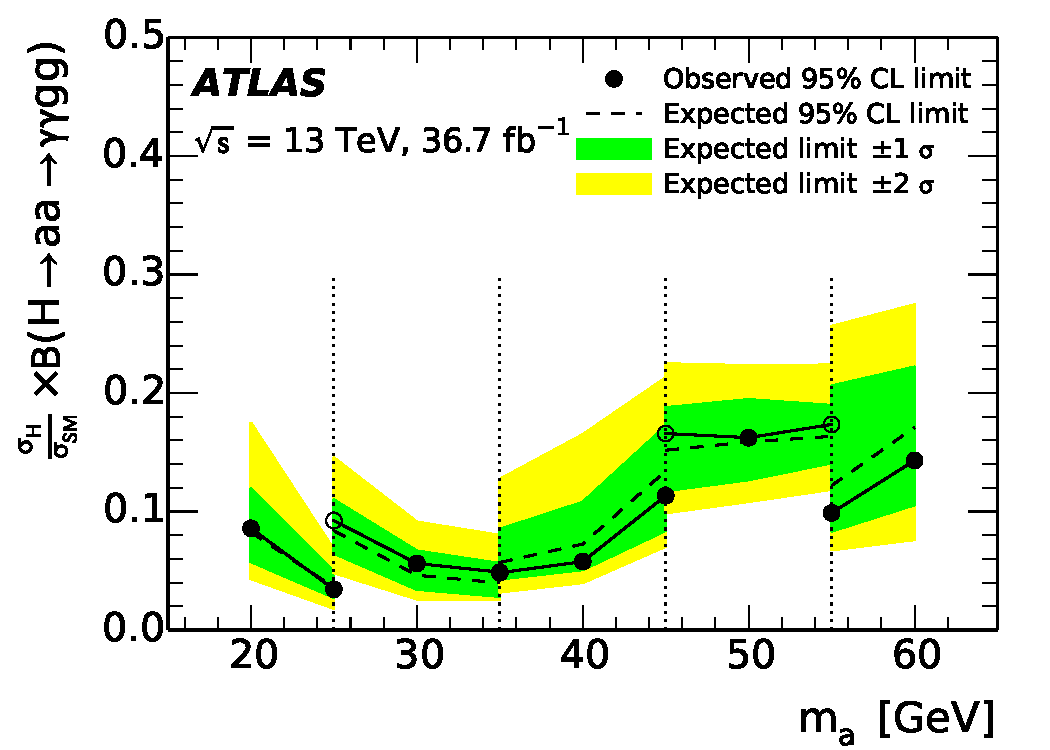
\includegraphics[width=0.9\textwidth]{figures/ABCD_twosigma_brazil_Freq_systs_obs_HF_ma_2_16_18.pdf}}
  \caption{The observed (solid line) and expected (dashed line) 95\% CL exclusion upper limit on 
    the \mbox{$pp\to H\to aa \to \gamma\gamma gg$} cross-section times branching ratio as a function of $m_a$,
    normalised to the SM inclusive $pp\to H$ cross-section~\cite{deFlorian:2016spz}.
  The vertical lines indicate the boundaries between the different $m_{\gamma\gamma}$ analysis regimes.
  At the boundaries, the $m_{\gamma\gamma}$ regime that yields the best expected limit is used to provide the observed exclusion limit (filled circles); the observed limit provided by the regime that yields the worse limit is also indicated (empty circles).
}
  \label{fig:brazil_ma}
\end{figure}

\section{Conclusions}

In summary, a search for exotic decays of the Higgs boson into a pair of new (pseudo)scalar particles,
$H\to aa$, in final states with two photons 
and two jets is conducted using 36.7~\ifb{} of $pp$ collisions at $\sqrt{s}=13$ \TeV{} recorded 
with the ATLAS detector at the LHC. The search for $H\to aa \to \gamma\gamma gg$ is performed
in the mass range $20 < m_a < 60~\GeV{}$ and with additional jet requirements 
to enhance VBF-produced signal while suppressing the $\gamma\gamma$+jets background.
No significant excess of data is observed relative to the SM predictions. An upper limit
is set for the product of the production cross-section for $pp\to H$ and the branching
ratio for the decay $H\to aa\to\gamma\gamma gg$. The upper limit ranges from 3.1 pb to 9.0 pb depending
on $m_a$, and is mostly driven by the statistical uncertainties.
These results complement the previous upper limit on $H\to aa\to\gamma\gamma\gamma\gamma$ and
further constrains the BSM parameter space for exotic decays of the Higgs boson.

%Another challenge present in this analysis is identifying and labeling the jets in the event as coming from the final state gluons, the quarks from the VBF production, or from pileup or underlying event.
%Tackling this challenge will involve utilizing newly developed techniques in quark-gluon tagging and pileup mitigation, including in the particularly difficult forward region of the calorimeter.
%Particularly challenging is the low-$m_a$ regime of the parameter space;
%in this regime, the gluons produced from the $a$ decay tend to be collimated and therefore can be reconstructed inside a single jet.
%Specific techniques will have to be developed in order to separate these gluons using custom substructure and track-based jet algorithms.
%
